\graphicspath{{Chapters/CrossSection/Figures/}}
\chapter{Observed Events and Cross Section Measurement}
\label{chap:CrossSection}

\section{Observed Events}

The expected and observed event yields are shown
in~\table{obs-expected-events-seven} for the 7~\tev\ analysis and
in~\table{obs-expected-events-eight} for the 8~\tev\ analysis. ~\fig{

%% Expected and observed events, 7 TeV
\begin{table}
\centering
\small
  \begin{tabular}{lcccc}
    \hline\hline
     7~\tev, \ZZ             & \eeee & \mmmm & \eemm & \llll \\
     \hline
Observed & 16 & 23 & 27 & 66 \\
Exp. Signal &   10.3 $\pm$ 0.1 $\pm$ 1.0 &  16.5 $\pm$ 0.2 $\pm$ 0.9 &  26.7 $\pm$ 0.2 $\pm$ 1.7 &  53.4 $\pm$ 0.3 $\pm$ 3.2 \\
Exp. Bg. & 0.5 $\pm$ 0.6 $\pm$ 0.3 & $<0.6$ & 0.7 $\pm$ 0.7 $\pm$ 0.6 & 0.9 $\pm$ 1.1 $\pm$ 0.7 \\
\hline\hline
    \\
    \hline\hline
     7~\tev, \ZZs             & \eeee & \mmmm & \eemm & \llll \\
     \hline
Observed & 21 & 30 & 33 & 84 \\
Exp. Signal &  12.3 $\pm$ 0.2 $\pm$ 1.2 &  20.5 $\pm$ 0.2 $\pm$ 1.1 &  31.6 $\pm$ 0.3 $\pm$ 2.0 &  64.4 $\pm$ 0.4 $\pm$ 4.0 \\
Exp. Bg. & 4.3 $\pm$ 1.4 $\pm$ 0.6 & $<0.9$ & 5.8 $\pm$ 1.6 $\pm$ 0.9 & 9.1 $\pm$ 2.3 $\pm$ 1.3 \\
    \hline\hline
  \end{tabular}

  \caption[Expected and observed events in 7~\tev\ data.]{\label{tab:obs-expected-events-seven}
           Number of expected and observed \ZZllll and \ZZsllll\ candidate events in
           7~\tev\ data, as well as the total data-drive background estimates,
       for the individual decay modes and for their combination.
       The first uncertainty is statistical while the second is systematic;
       uncertainties on the integrated luminosity (3.9\%) are not included.
          }
\end{table}

%% Expected and observed events, 8 TeV
\begin{table}
\centering
\small
  \begin{tabular}{lcccc}
    \hline\hline
     7~\tev, \ZZ             & \eeee & \mmmm & \eemm & \llll \\
     \hline
Observed & \ZZEightTeVNObsZZEEEE & \ZZEightTeVNObsZZMMMM & \ZZEightTeVNObsZZEEMM & \ZZEightTeVNObsZZEELL \\
Exp. Signal &   
    \measStatSystSym{\ZZEightTeVNExpZZEEEE}{\ZZEightTeVNExpStatZZEEEE}{\ZZEightTeVNExpStatZZEEEE} & 
    \measStatSystSym{\ZZEightTeVNExpZZMMMM}{\ZZEightTeVNExpStatZZMMMM}{\ZZEightTeVNExpStatZZMMMM} & 
    \measStatSystSym{\ZZEightTeVNExpZZEEMM}{\ZZEightTeVNExpStatZZEEMM}{\ZZEightTeVNExpStatZZEEMM} & 
    \measStatSystSym{\ZZEightTeVNExpZZLLLL}{\ZZEightTeVNExpStatZZLLLL}{\ZZEightTeVNExpStatZZLLLL} \\
Exp. Bg. & 
    \measStatSystSym{\ZZEightTeVNBgZZEEEE}{\ZZEightTeVNBgStatZZEEEE}{\ZZEightTeVNBgStatZZEEEE} & 
    \measStatSystSym{\ZZEightTeVNBgZZMMMM}{\ZZEightTeVNBgStatZZMMMM}{\ZZEightTeVNBgStatZZMMMM} & 
    \measStatSystSym{\ZZEightTeVNBgZZEEMM}{\ZZEightTeVNBgStatZZEEMM}{\ZZEightTeVNBgStatZZEEMM} & 
    \measStatSystSym{\ZZEightTeVNBgZZLLLL}{\ZZEightTeVNBgStatZZLLLL}{\ZZEightTeVNBgStatZZLLLL} \\
\hline\hline
    \\
    \hline\hline
     7~\tev, \ZZs             & \eeee & \mmmm & \eemm & \llll \\
     \hline
Observed & 21 & 30 & 33 & 84 \\
Exp. Signal &  12.3 $\pm$ 0.2 $\pm$ 1.2 &  20.5 $\pm$ 0.2 $\pm$ 1.1 &  31.6 $\pm$ 0.3 $\pm$ 2.0 &  64.4 $\pm$ 0.4 $\pm$ 4.0 \\
Exp. Bg. & 4.3 $\pm$ 1.4 $\pm$ 0.6 & $<0.9$ & 5.8 $\pm$ 1.6 $\pm$ 0.9 & 9.1 $\pm$ 2.3 $\pm$ 1.3 \\
    \hline\hline
  \end{tabular}

  \caption[Expected and observed events in 7~\tev\ data.]{\label{tab:obs-expected-events-seven}
           Number of expected and observed \ZZllll and \ZZsllll\ candidate events in
           7~\tev\ data, as well as the total data-drive background estimates,
       for the individual decay modes and for their combination.
       The first uncertainty is statistical while the second is systematic;
       uncertainties on the integrated luminosity (3.9\%) are not included.
          }
\end{table}

% 2D plot, 7 TeV
% Use PDF figure as text alignment is off in eps
 \begin{figure}[htbp]
 \begin{center}
  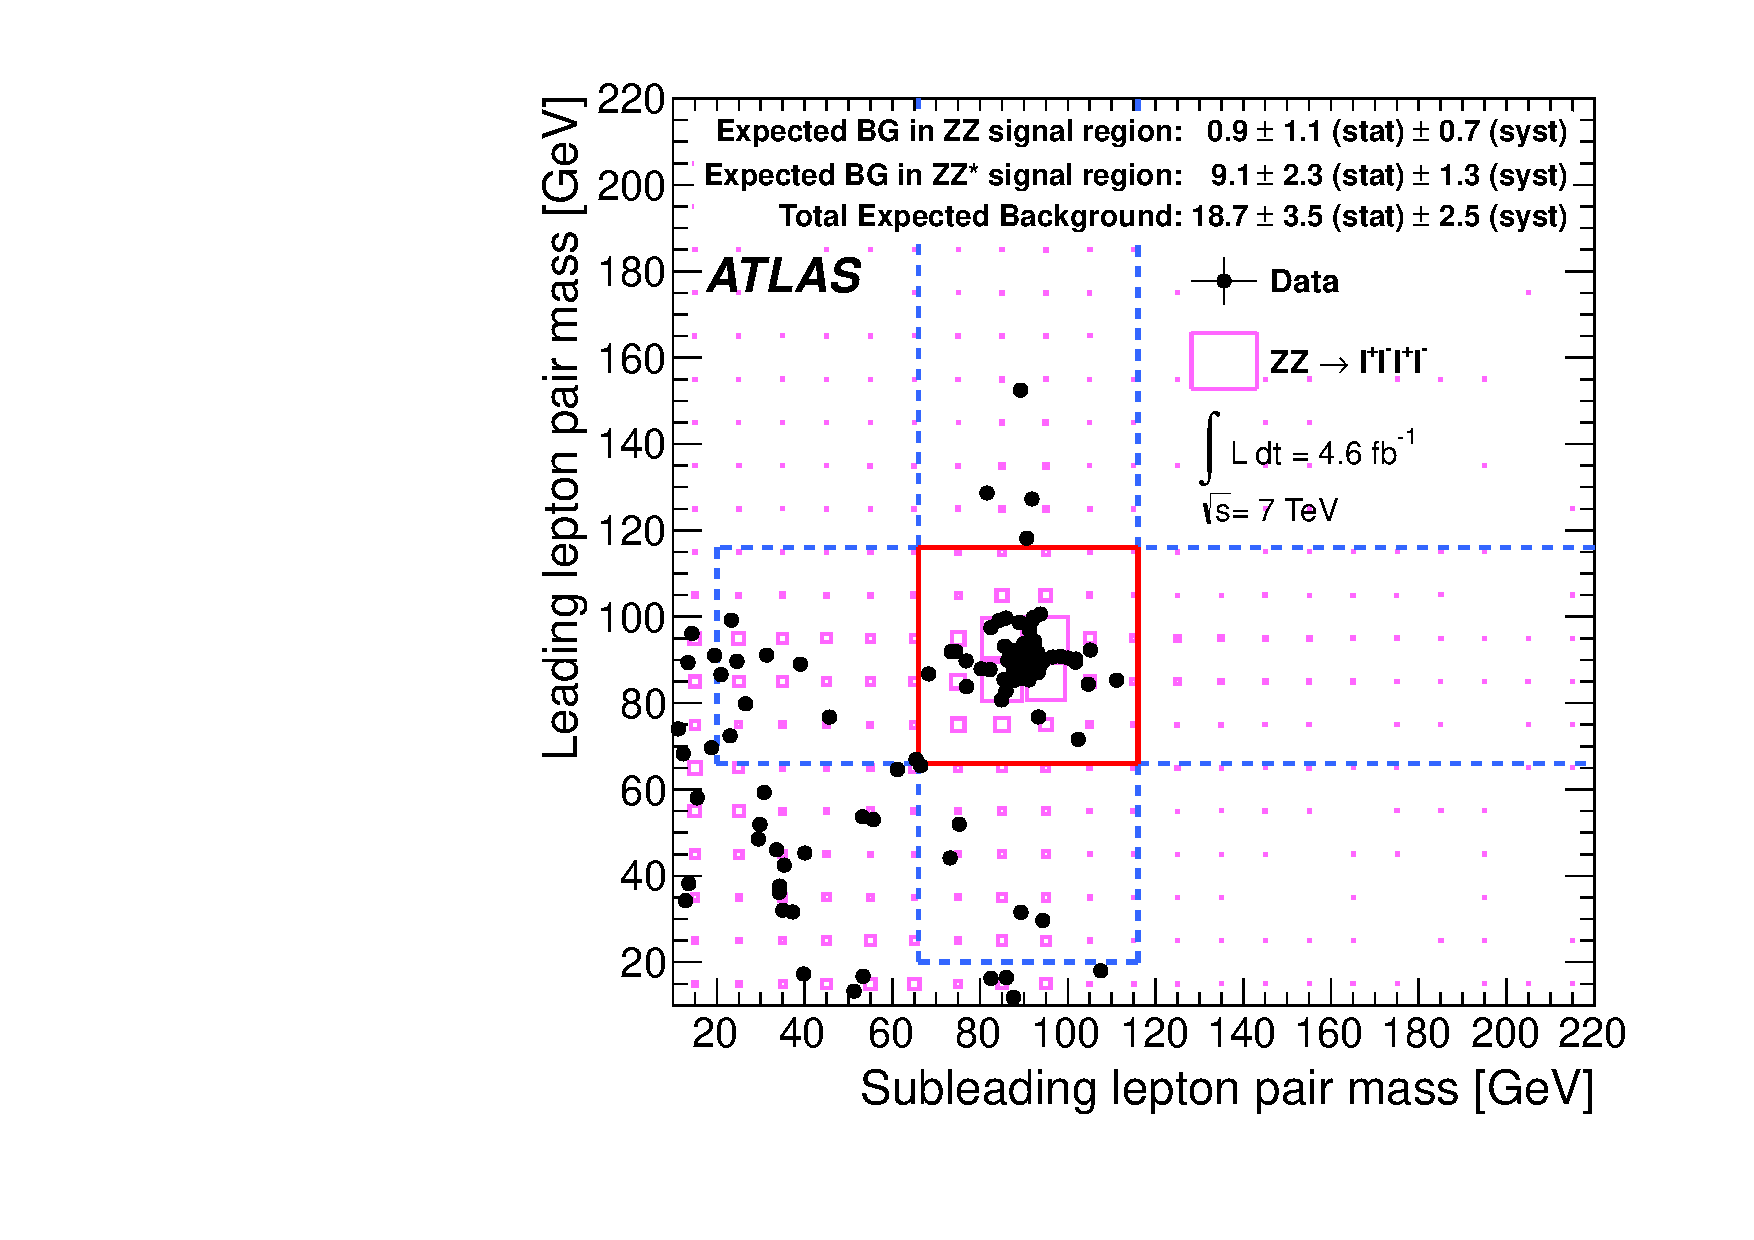
\includegraphics[width=0.7\textwidth]{7TeV/h_mz1_mz2.pdf}\hfill
  \caption[Mass of the leading \leppair versus the mass of the
  sub-leading \leppair for candidate events, passing all of the selection
  requirements apart from the \dilepton\ mass requirements, in the 7~\tev\ data.]
  {\small Mass of the leading \leppair versus the mass of the
  sub-leading \leppair for candidate events in the 7~\tev\ data after
  applying all of the selection
  requirements apart from the \dilepton\ mass requirements.
  The events observed in the data are shown as solid circles and the \ZZsllll\ signal prediction from simulation as boxes.
  The size of each box is proportional to the number of events in each bin.  
  The region enclosed by the solid (dashed) lines indicates the signal region defined by the
  \dilepton\ mass requirements on for \ZZ\ (\ZZs) events.
  %The background estimate is described in section 5.1.
   }
    \label{fig:zzdists-seven-Zmass}
 \end{center}
 \end{figure}

% pT_Z vs dR 7 TeV
 \begin{figure}[htbp]
 \begin{center}
  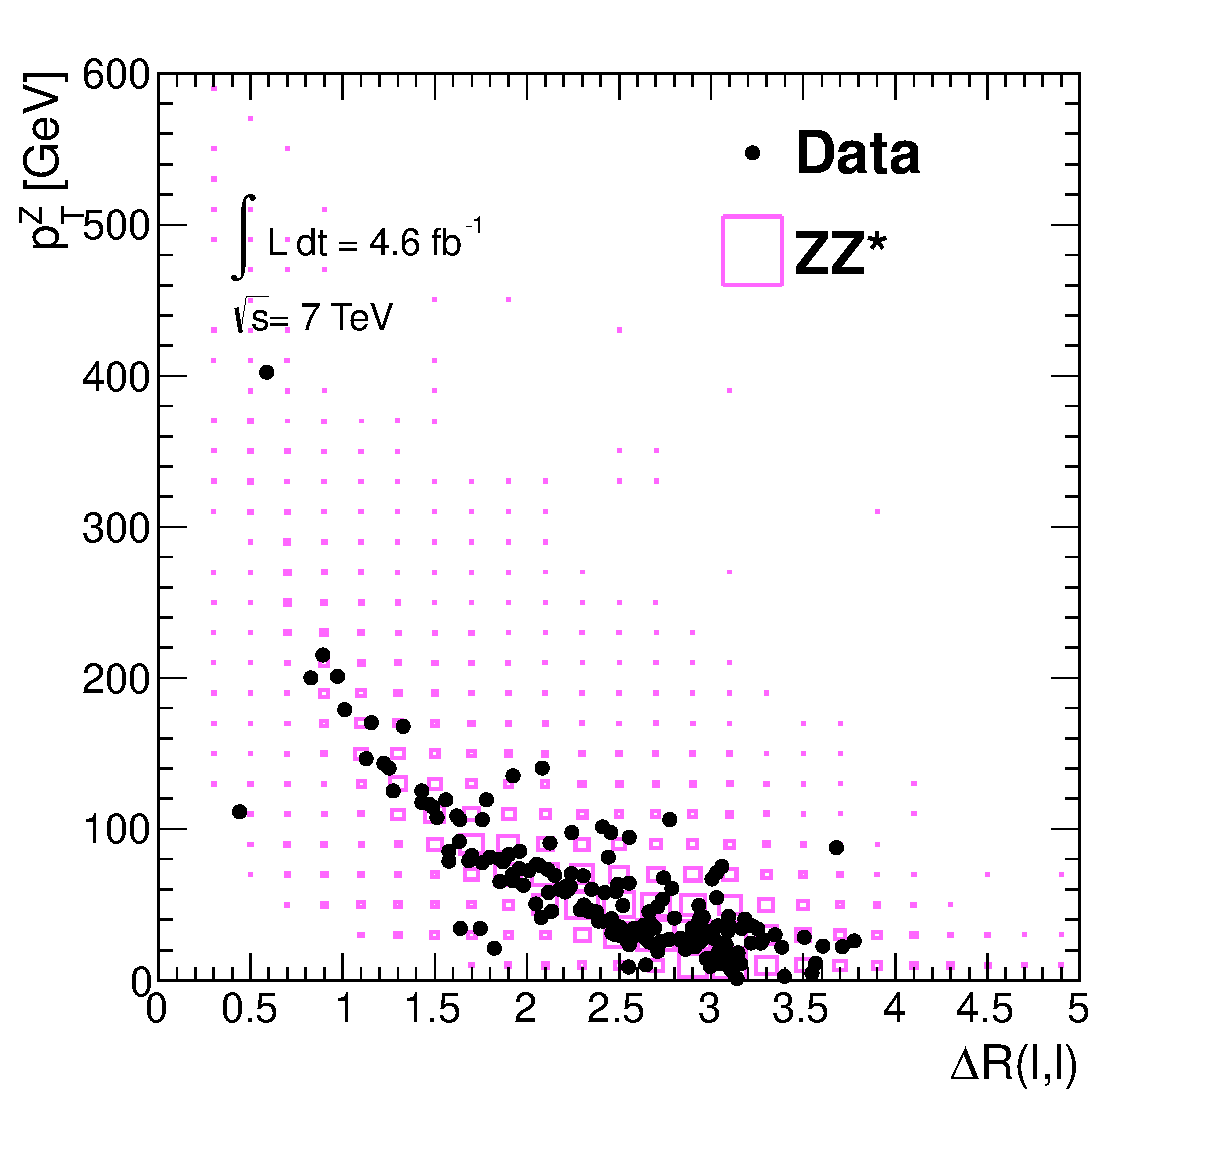
\includegraphics[width=0.7\textwidth]{7TeV/h_dr_ptz}\hfill
  \caption[Transverse momentum of the \leppair s versus the angle of the two leptons
    forming the pair for events passing the \ZZs\ selection in 7~\tev\ data.]
    {\small Transverse momentum of the \leppair s versus the angle of the two leptons
    forming the pair for events passing the \ZZs\ selection in 7~\tev\ data (two
    entries per event).}
 \label{fig:zzdists-dr-ptz1-seven}
 \end{center}
 \end{figure}

% m_ZZ vs min(dR) 7 TeV
 \begin{figure}[htbp]
 \begin{center}
  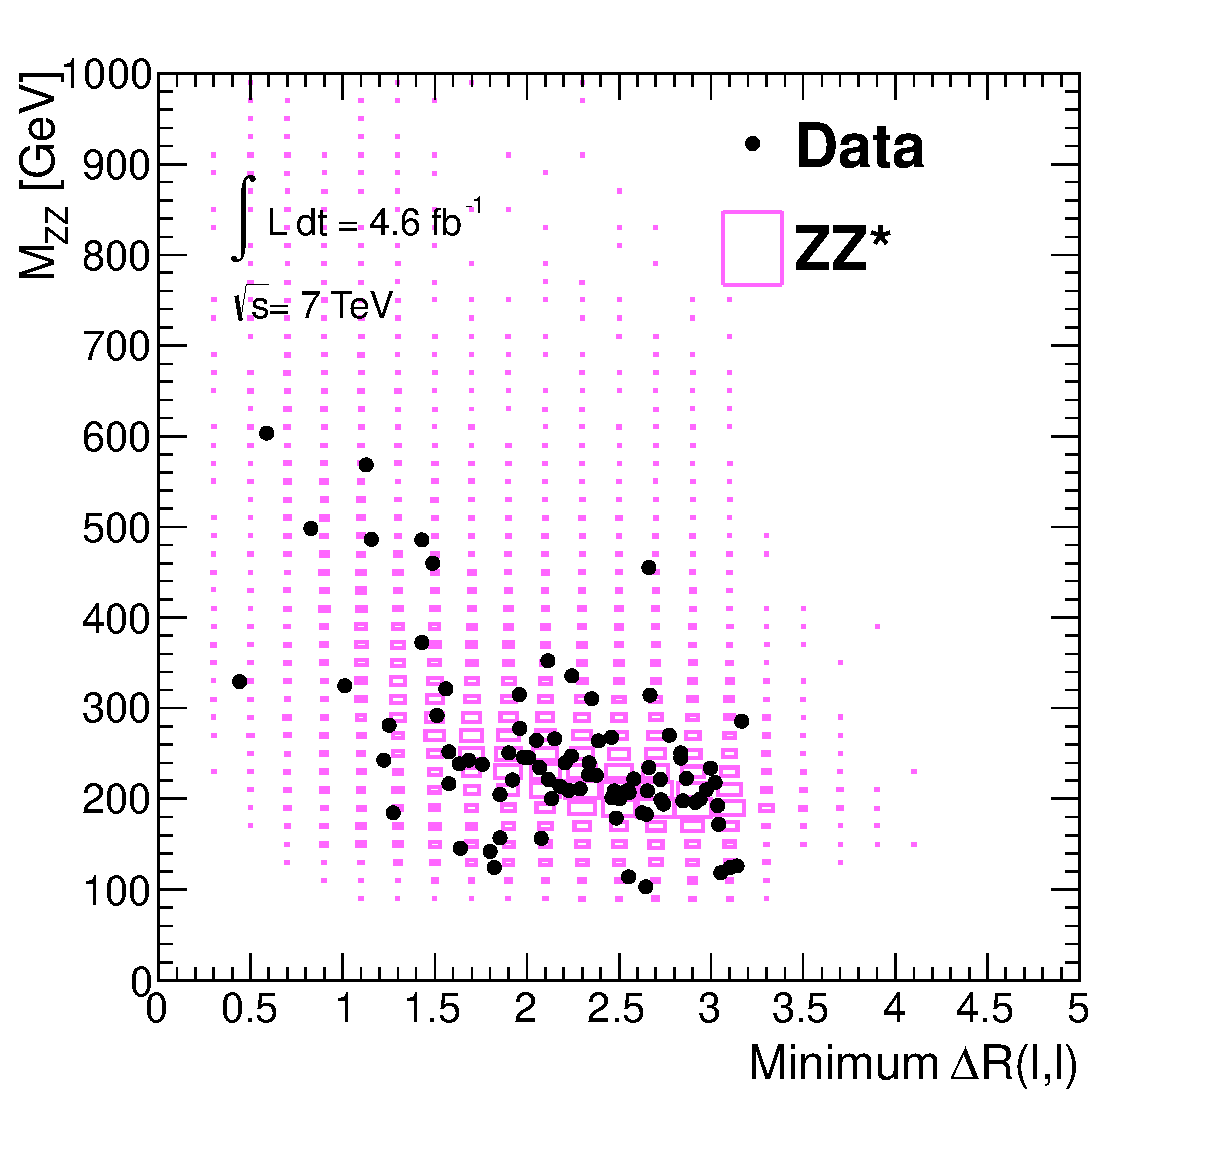
\includegraphics[width=0.7\textwidth]{7TeV/h_mindr_mzz}\hfill
  \caption[The invariant mass of the four lepton system \mZZ\ versus the
    minimum \deltaR\ between any pair of leptons in the event for events passing
    the \ZZs\ selection in 7~\tev\ data.]
    {\small The invariant mass of the four lepton system \mZZ\ versus the
    minimum \deltaR\ between any pair of leptons in the event for events passing
    the \ZZs\ selection in 7~\tev\ data.
    The events observed in the data are shown as black dots and the signal prediction as boxes.}
 \label{fig:zzdists-mindr-mzz-seven}
 \end{center}
 \end{figure}

\subsection{Kinematic Distributions}

% 7 TeV, Z1_m, Z2_m, m_Z>7GeV
\begin{figure}[htbp]
    \begin{center}
     \subfigure[]{
     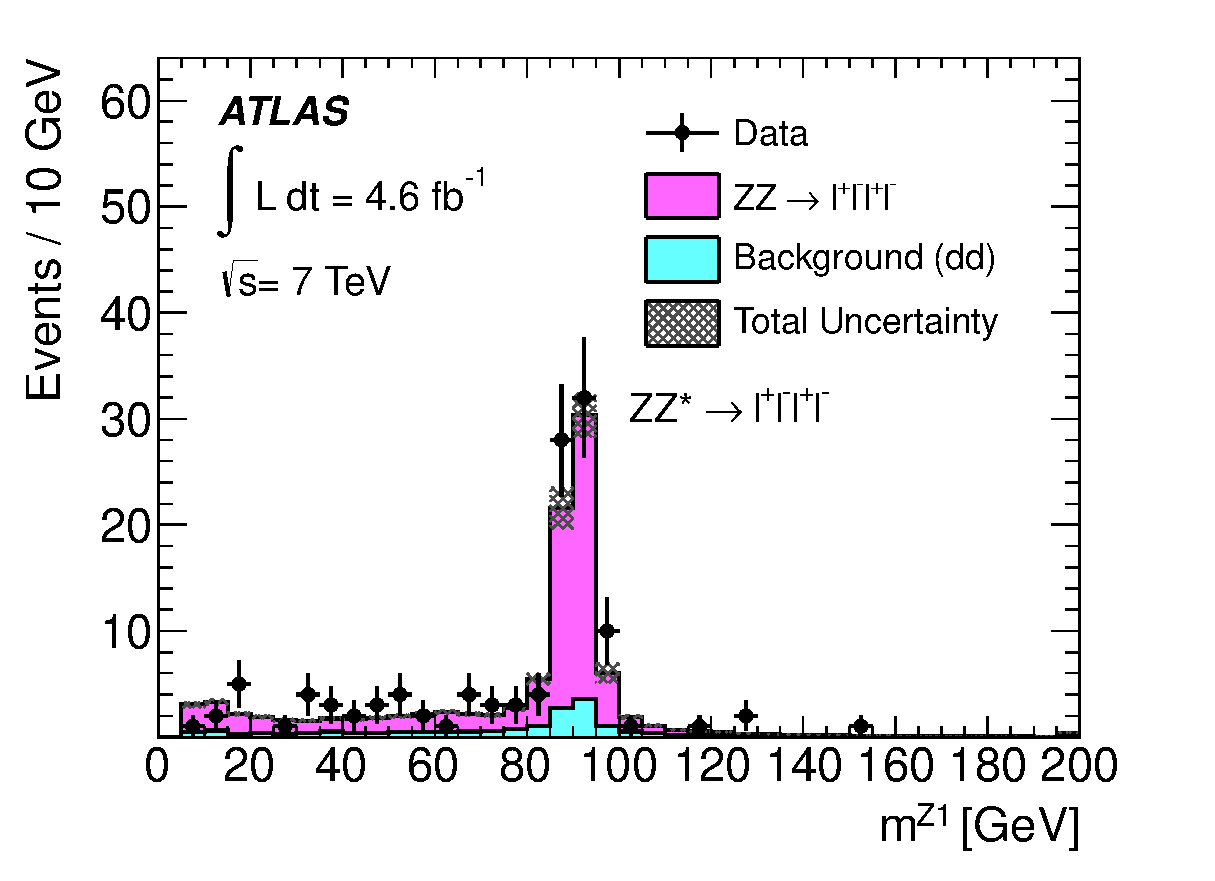
\includegraphics[width=0.47\textwidth]{7TeV/h_4l_ZZs_Z1_m}
     }
     \subfigure[]{
     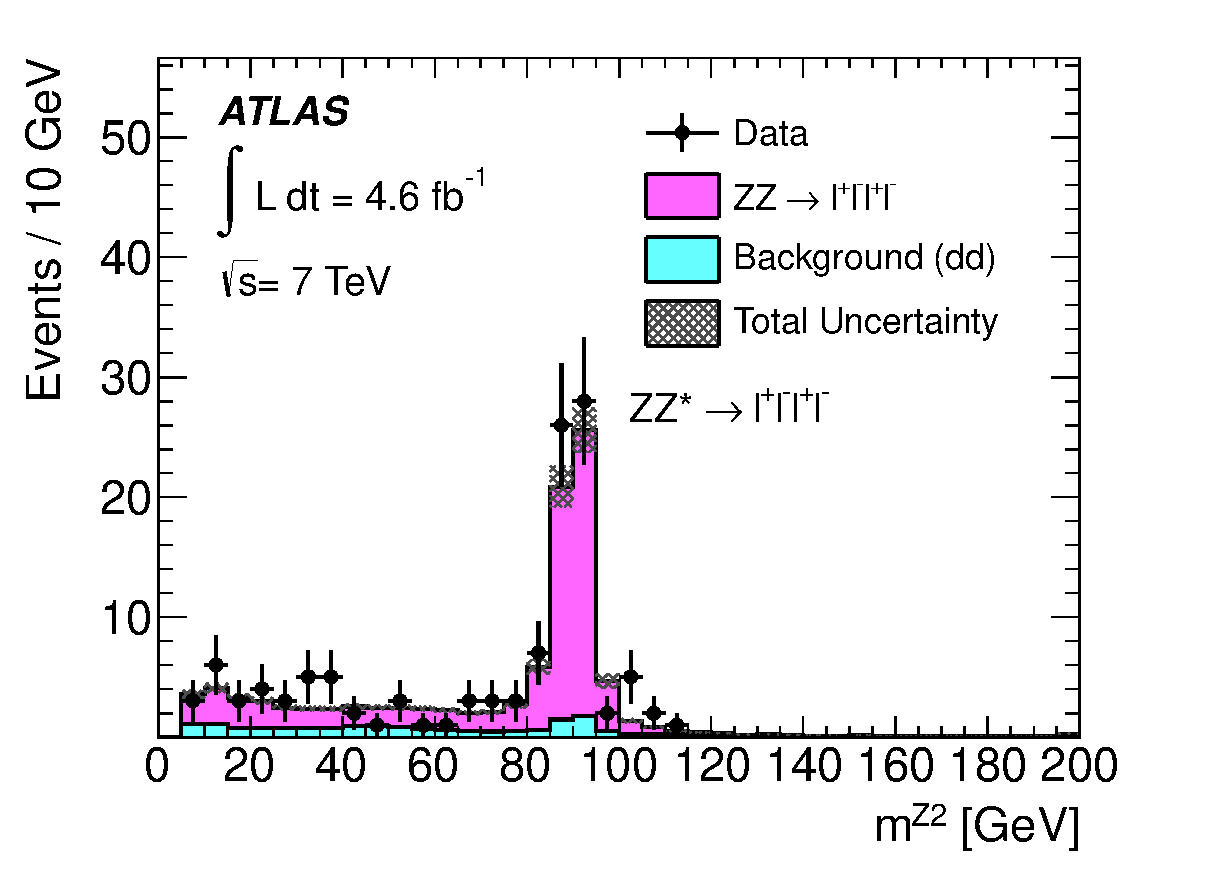
\includegraphics[width=0.47\textwidth]{7TeV/h_4l_ZZs_Z2_m}
     }
    \label{fig:zzdists-Zmass-seven}
    \caption[Invariant masses of the (a) leading and (b) subleading \leppair
    in candidate \ZZ\ events in the 7~\tev\ data.]
    {Invariant masses of the (a) leading and (b) subleading \leppair
    in candidate \ZZ\ events in the 7~\tev\ data. Both \leppair s are required to have
    $m_{\ell\ell}>7$~\gev.  The points represent the observed data and the
    histograms show the prediction from simulation, where the background is
    normalized to the data-driven estimate as described in
    ~\chap{BackgroundEsitmate}. The shaded band shows the combined statistical and
    systematic uncertainty on the prediction. 
}
\end{center}
\end{figure}

% 7 TeV, ZZ, ZZ_pt / ZZ_m
\begin{figure}[htbp]
    \begin{center}
     \subfigure[]{
     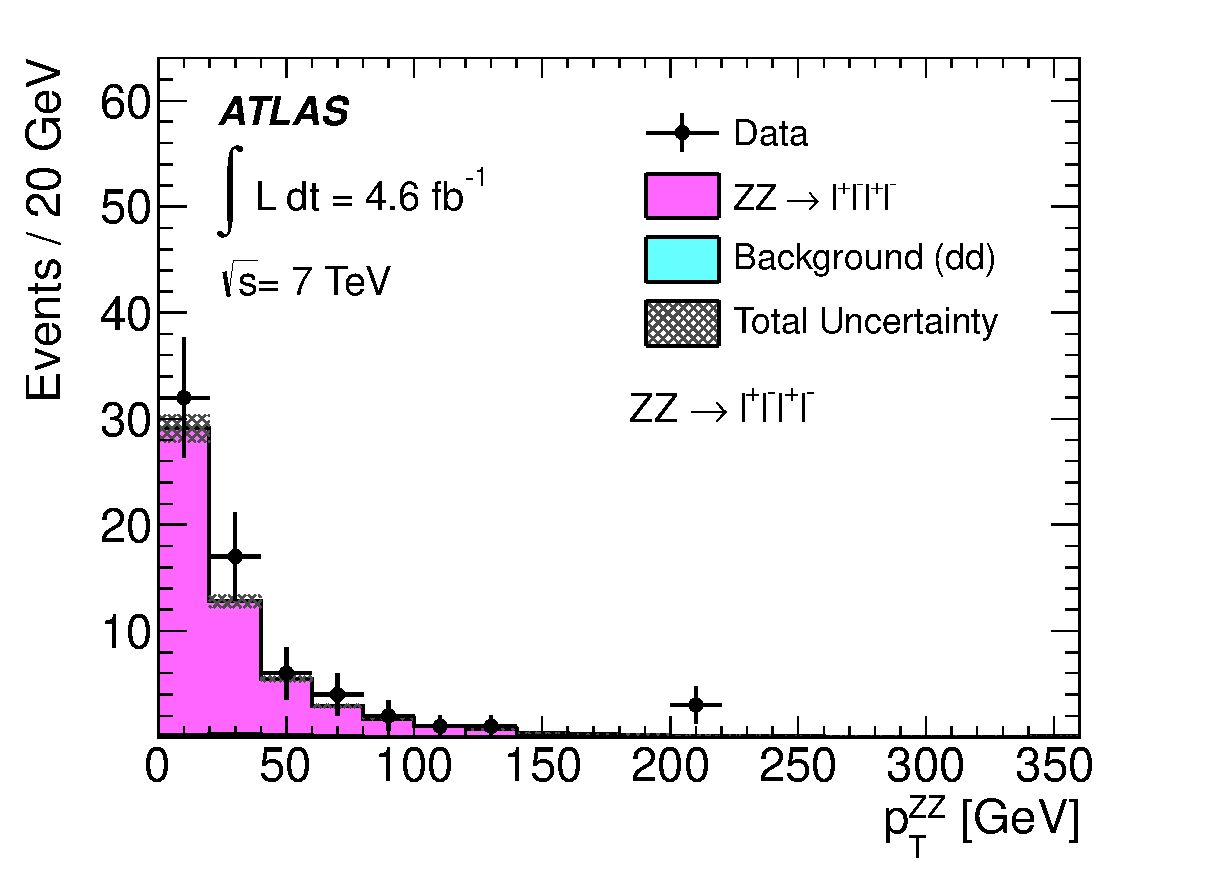
\includegraphics[width=0.47\textwidth]{7TeV/h_4l_ZZ_ZZ_pt}
     }
     \subfigure[]{
     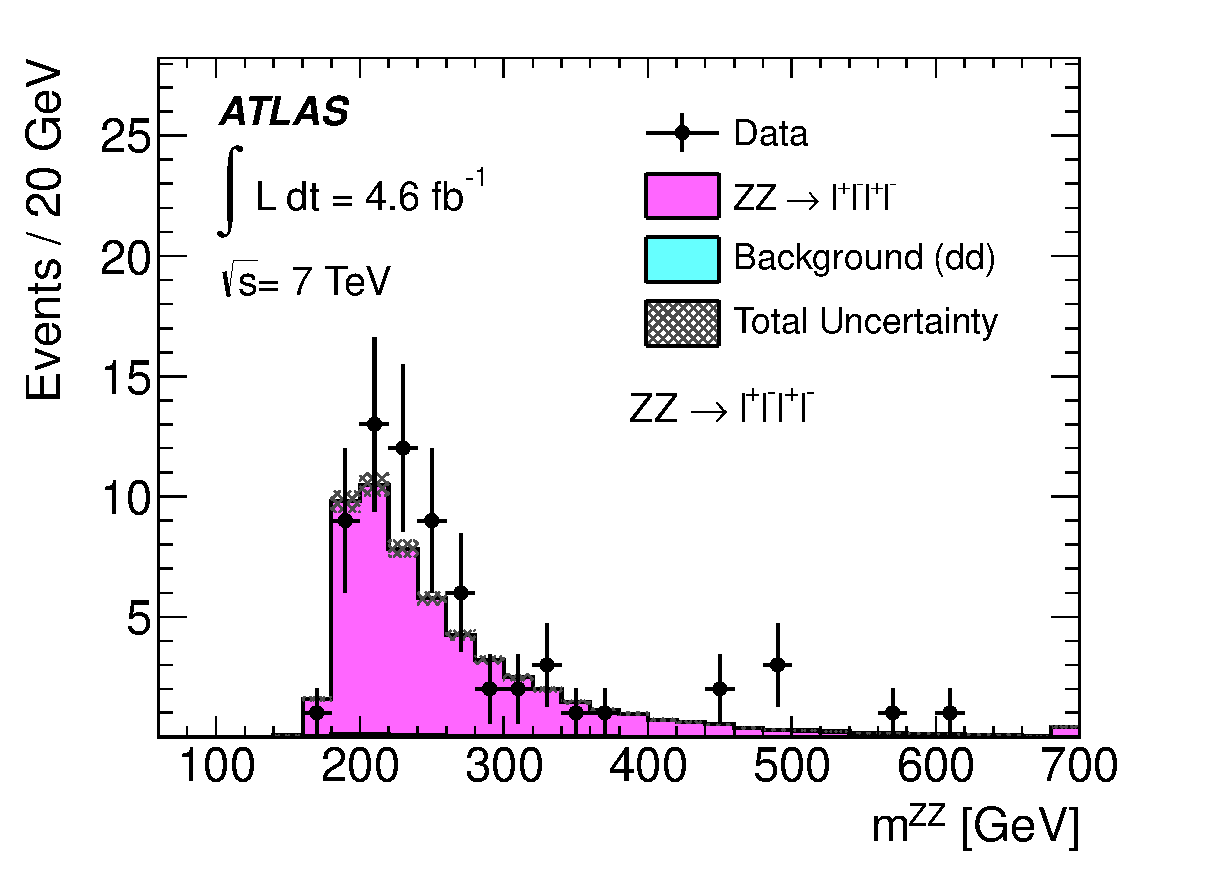
\includegraphics[width=0.47\textwidth]{7TeV/h_4l_ZZ_ZZ_m}
     }
     \subfigure[]{
     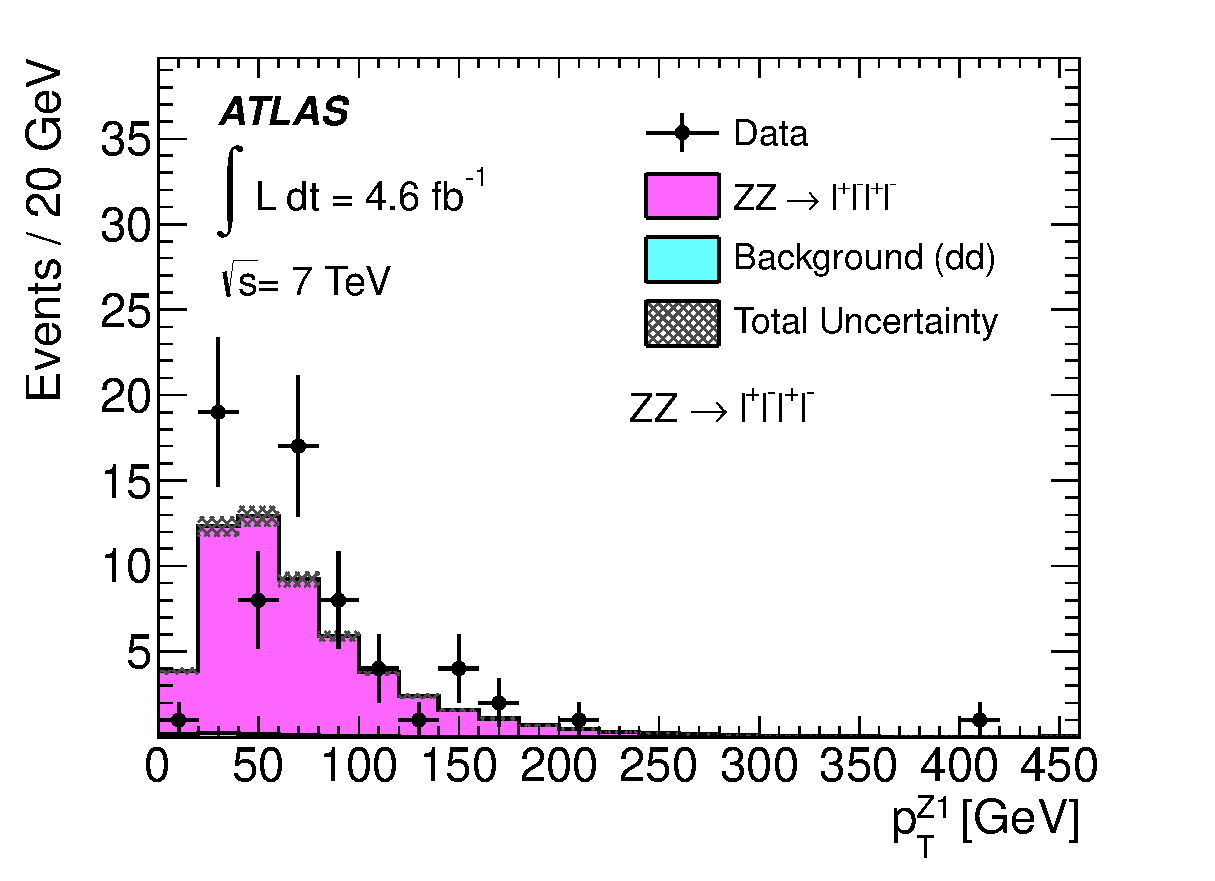
\includegraphics[width=0.47\textwidth]{7TeV/h_4l_ZZ_Z1_pt}
     }
     \subfigure[]{
     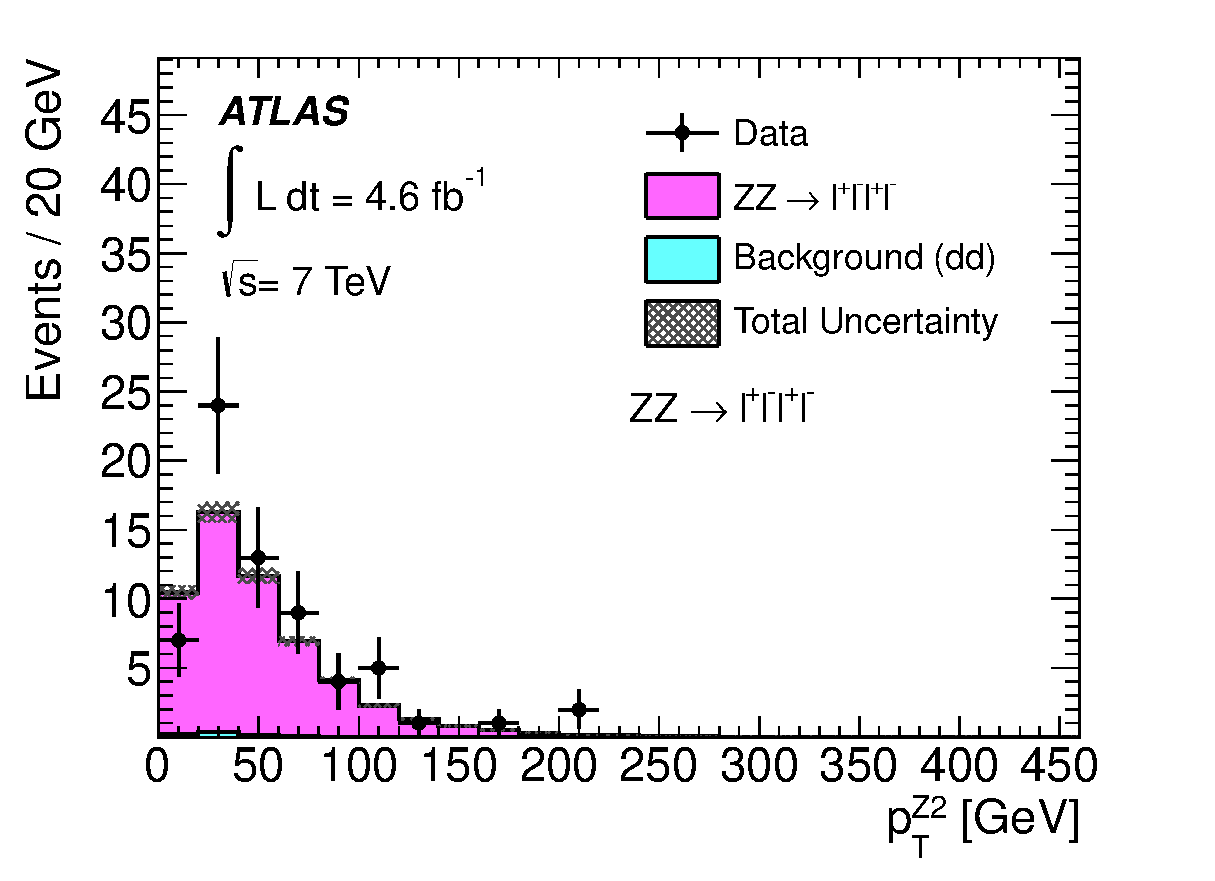
\includegraphics[width=0.47\textwidth]{7TeV/h_4l_ZZ_Z2_pt}
     }
    \label{fig:zzdists-ZZ-seven}
    \caption[Kinematic distributions for events passing the \ZZ\ selection in
    the 7~\tev\ data.]
    {Kinematic distributions for events passing the \ZZ\ selection in
    the 7~\tev\ data: (a) transverse momentum $\pT^{\ZZ}$ and (b) invariant mass $m^{\ZZ}$ of the 
    four-lepton system, (c) transverse momentum of the leading
    dilepton pair $\pt^{Z1}$, and (d) transverse momentum of the subleading
    dilepton pair $\pt^{Z2}$. The points represent the observed data and the 
    histograms show the prediction from simulation, where the background
    is normalized to the data-driven (dd) estimate as described in ~\chap{BackgroundEsitmate}. The shaded band 
    shows the combined statistical and systematic uncertainty on the prediction. 
    }
    \end{center}
\end{figure}

% 7 TeV, ZZ*, ZZ_pt / ZZ_m
\begin{figure}[htbp]
\begin{center}
    \subfigure[]{
    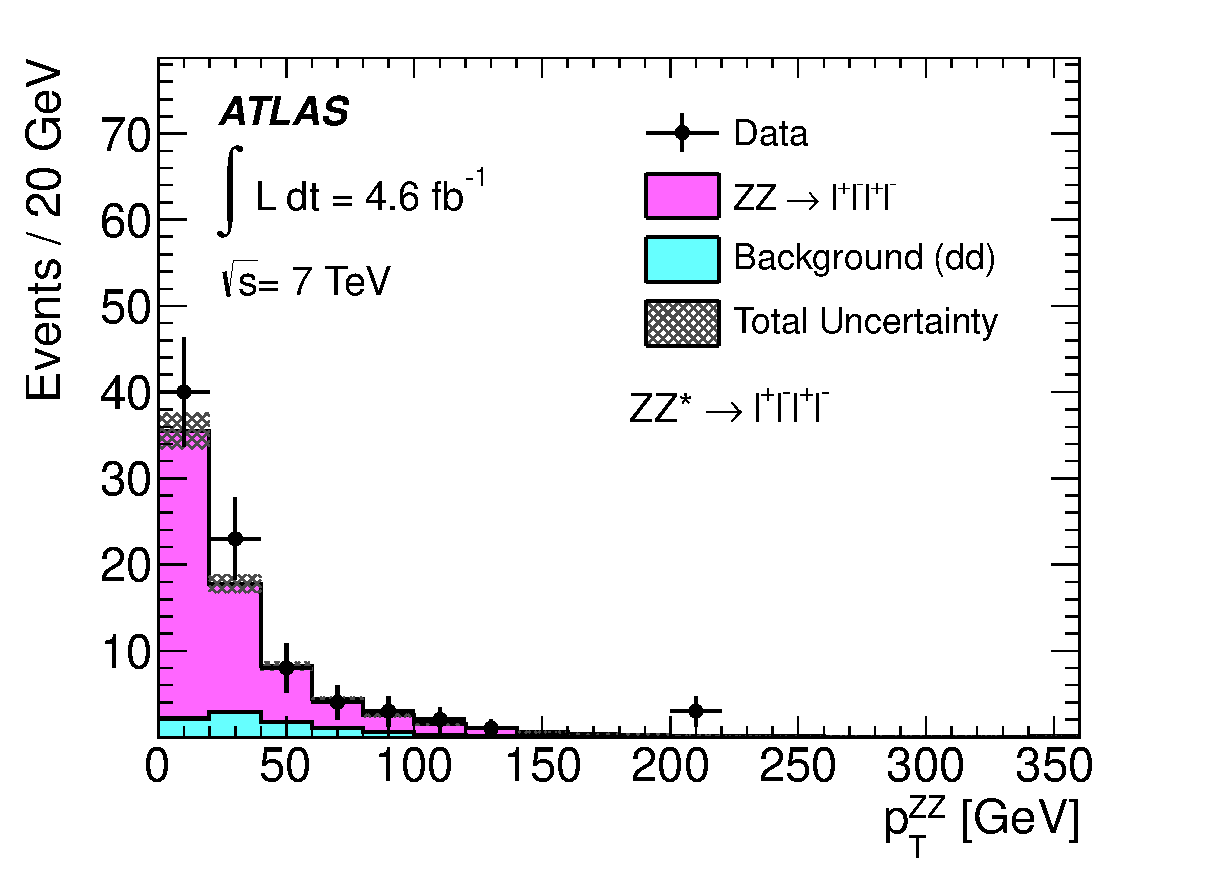
\includegraphics[width=0.47\textwidth]{7TeV/h_4l_ZZs_ZZ_pt}
    }
    \subfigure[]{
    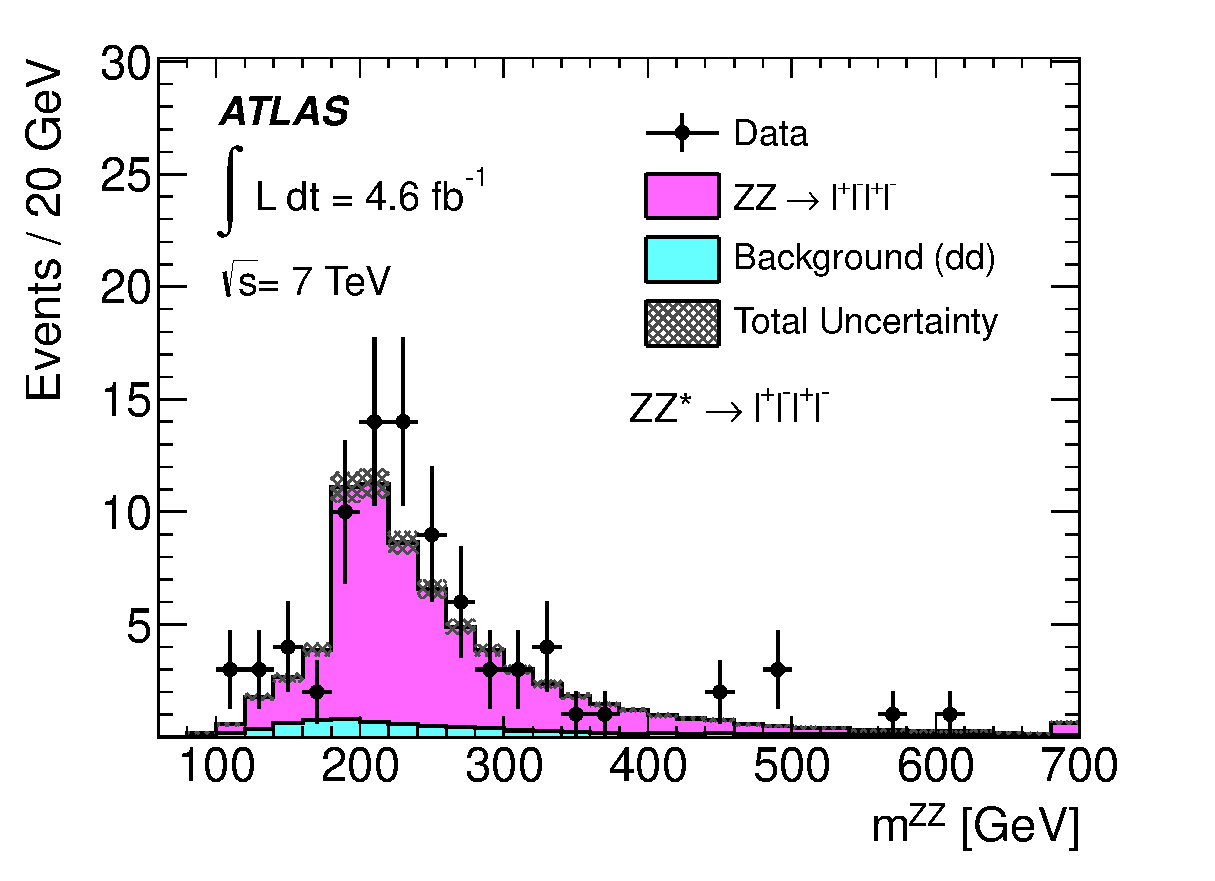
\includegraphics[width=0.47\textwidth]{7TeV/h_4l_ZZs_ZZ_m}
    }
    \subfigure[]{
    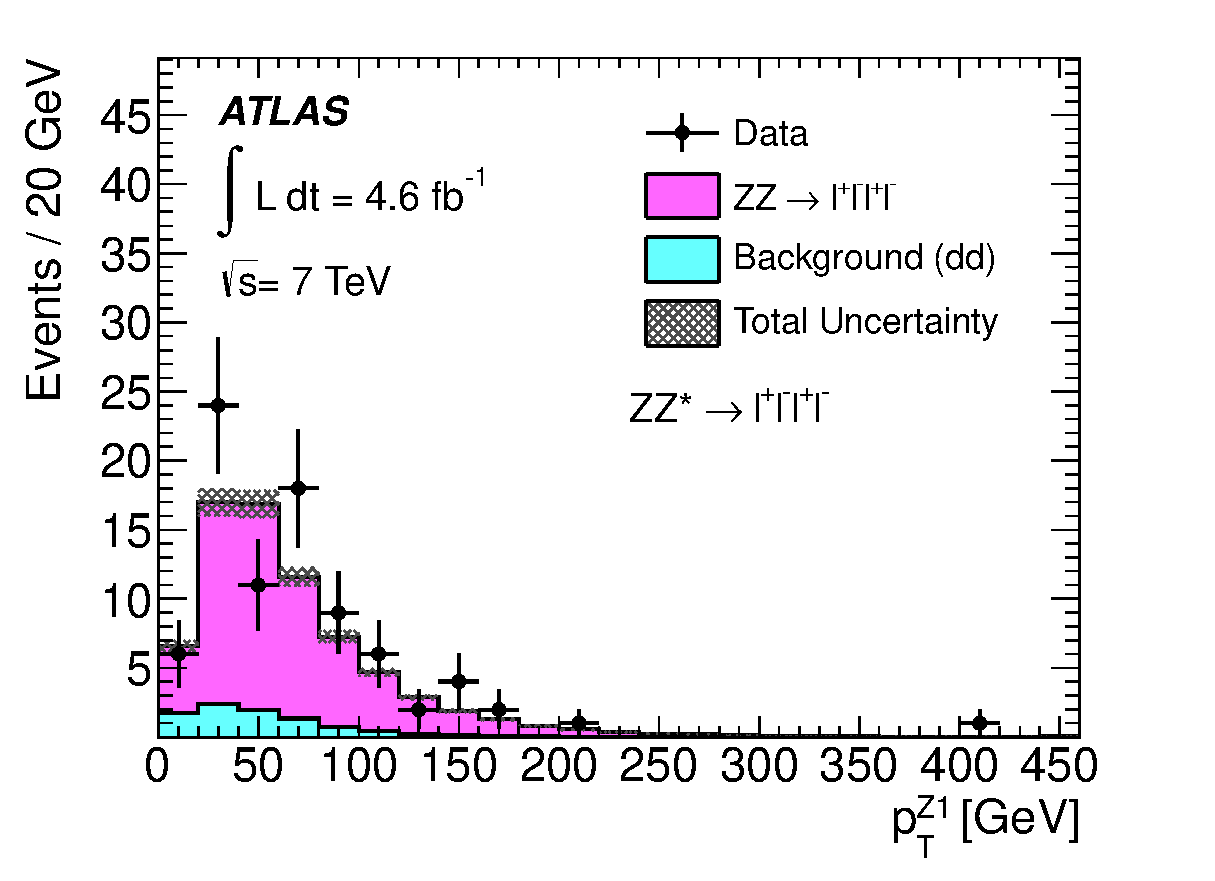
\includegraphics[width=0.47\textwidth]{7TeV/h_4l_ZZs_Z1_pt}
    }
    \subfigure[]{
    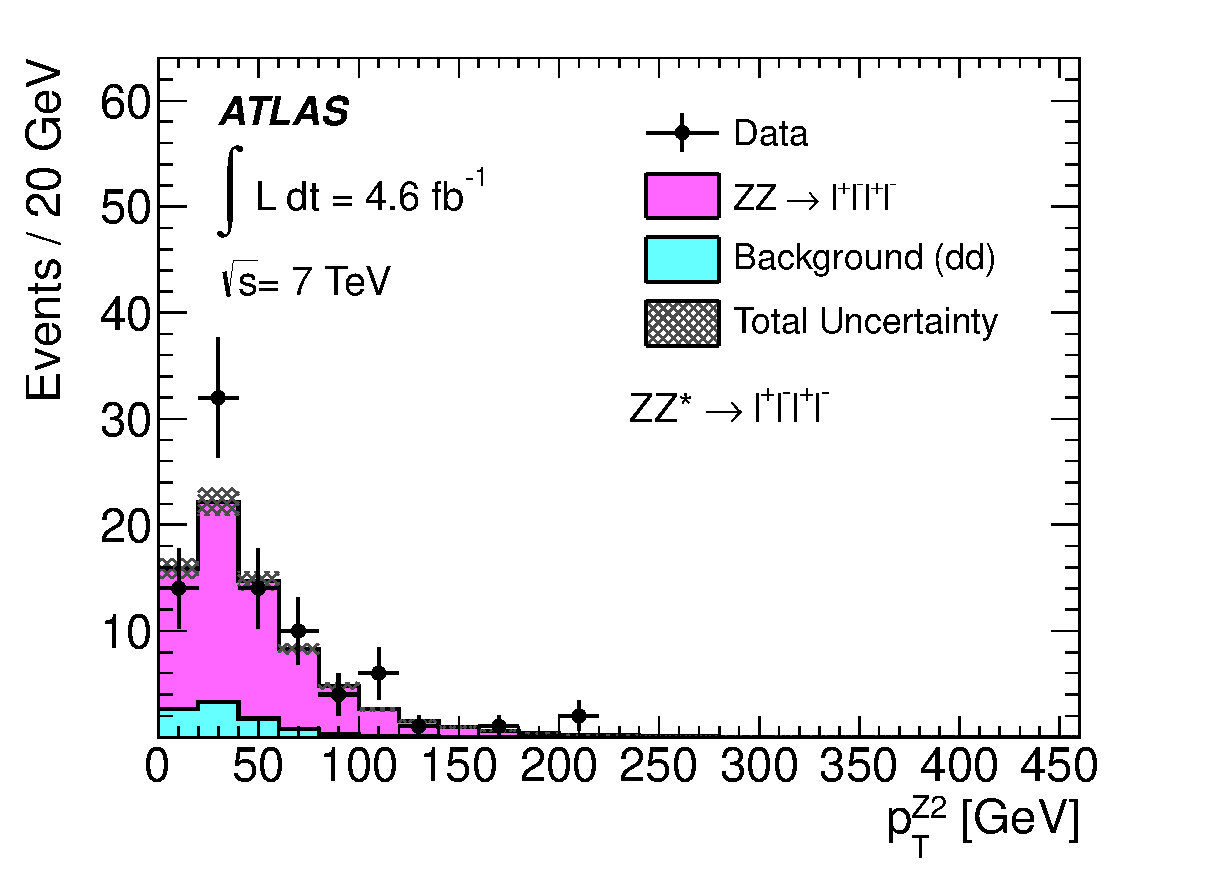
\includegraphics[width=0.47\textwidth]{7TeV/h_4l_ZZs_Z2_pt}
    }
    \label{fig:zzdists-ZZs-seven}
    \caption[Kinematic distributions for events passing the \ZZs\ selection in
    the 7~\tev\ data.]
    {Kinematic distributions for events passing the \ZZs\ selection in
    the 7~\tev\ data: (a) transverse momentum $\pT^{\ZZ}$ and (b) invariant mass $m^{\ZZ}$ of the 
    four-lepton system, (c) transverse momentum of the leading
    dilepton pair $\pt^{Z1}$, and (d) transverse momentum of the subleading
    dilepton pair $\pt^{Z2}$. The points represent the observed data and the 
    histograms show the prediction from simulation, where the background
    is normalized to the data-driven (dd) estimate as described in ~\chap{BackgroundEsitmate}. The shaded band 
    shows the combined statistical and systematic uncertainty on the prediction. 
    }
\end{center}
\end{figure}

\section{Cross Section Measurement}
\subsection{Cross Section Definition}
\subsection{Fiducial Acceptance}
\subsection{Cross Section Extraction}
